%%%%%%%%%%%%%%%%%%%%%%%%%%%%%%%%%%%%%%%%%%%%%%%%%%%%%%%%%%%%%%%%%%%%%%%%
%                                                                      %
%     File: Thesis_Appendix.tex                                        %
%     Tex Master: Thesis.tex                                           %
%                                                                      %
%     Author: Andre C. Marta                                           %
%     Last modified : 21 Jan 2011                                      %
%                                                                      %
%%%%%%%%%%%%%%%%%%%%%%%%%%%%%%%%%%%%%%%%%%%%%%%%%%%%%%%%%%%%%%%%%%%%%%%%

\chapter{User Survey}
\label{chapter:appendixVectors}

We asked some people to answer a survey and we got 30 answers that helped us understand photography related habits and user wishes, and compiled them in this appendix.

\section{User characterization}

Our survey started by asking the respondents to describe themselves and their libraries.


\subsubsection{Kind of Photographer} % (fold)
\label{ssub:subsubsection_name}


\begin{wrapfigure}{r}{0.3\textwidth}
	\vspace{-20pt}
	\begin{center}
		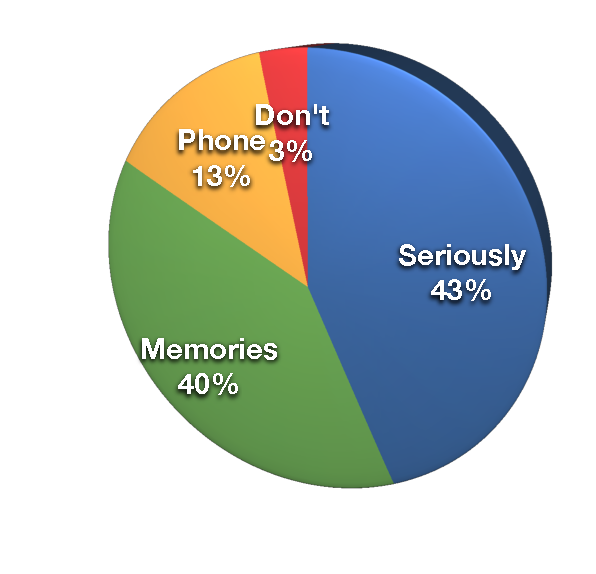
\includegraphics[width=\linewidth]{Figures/survey/desc}
	\end{center}
	\vspace{-20pt}
	\caption{Kinds of photographers.}
	\vspace{-5pt}
	\label{fig:us:desc}
\end{wrapfigure}

We asked the respondents what of the following options described them the best:

\begin{myitemize}
	\item I'm a \textbf{professional} photographer.
	\item I like to take photography \textbf{seriously} but I'm no professional.
	\item I like to take pictures just to keep as \textbf{memories}, but I'm not a photo-geek.
	\item I only use my camera \textbf{phone} for fun.
	\item I \textbf{don't} take pictures.
\end{myitemize}

As we can see on \fig{us:desc}, most respondents like photography and take photos, being mostly people who take photos for memories and people who are really into photography but are not professionals.

% subsubsection subsubsection_name (end)





\subsubsection{Storage of digital photos} % (fold)
\label{ssub:storage_of_digital_photos}
The second question was a check to verify if the respondents stored digital photos in their computers. The questionnaire would end if they said no. Fortunately, everyone said yes.
% subsubsection storage_of_digital_photos (end)





\section{Characterization of Photo Library} % (fold)
\label{sec:characterization_of_photo_library}

\begin{wrapfigure}{r}{0.5\textwidth}
	\vspace{-20pt}
	\begin{center}
		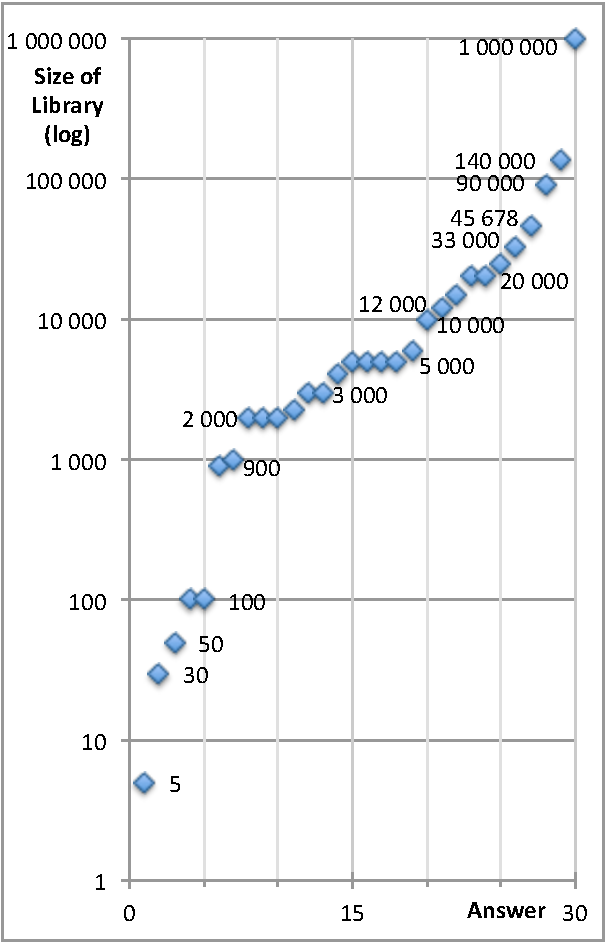
\includegraphics[width=\linewidth]{Figures/survey/libsize}
	\end{center}
	\vspace{-20pt}
	\caption{Library Size}
	\vspace{-70pt}
	\label{fig:us:desc}
\end{wrapfigure}

We then inquired about their photo libraries.
\vspace{\baselineskip}

\subsubsection{Library size} % (fold)
\label{ssub:library_size}

To start the survey about the library, we inquired how large was the respondents photo library.

We made this an open question, because we wanted to obtain real values from the users and not just limiting to a number of options that hardly represent anything. The answers for this question can be seen on \fig{us:desc}.

We were surprised by the values we got, going from 5 up to a million photos.

Almost half of the answers are between the 1 \nolinebreak 000 and the 10 000 values, having two thirds of the results falling between 0 and 10 000. We also found the median value of the answers, which is 5 \nolinebreak 000.

% subsubsection library_size (end)


\vspace{3\baselineskip}

\begin{wrapfigure}{r}{0.3\textwidth}
	\vspace{-20pt}
	\begin{center}
		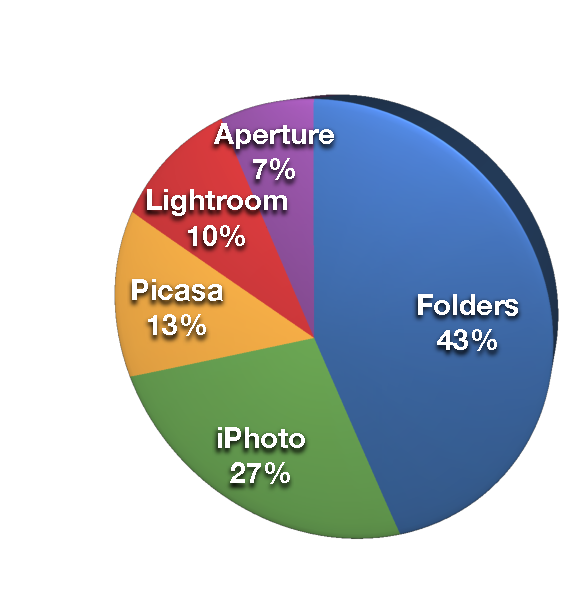
\includegraphics[width=\linewidth]{Figures/survey/sw}
	\end{center}
	\vspace{-20pt}
	\caption{Software used}
	\vspace{-5pt}
	\label{fig:us:desc}
\end{wrapfigure}

\subsubsection{Usage of Software} % (fold)
\label{ssub:usage_of_software}

We then questioned about what software applications did people use to help them organize their collections. Almost half admitted they only used folders for their organization, while the other 17 people used some kind of software.

Going through each software applications, we can see that 40\% use an entry-level software (iPhoto and Picasa) while 17\% prefer more Pro-level systems.

We tried to correlate the size of the collections with the software used but we realized that we probably don't have enough data for some of those softwares and that users might not have their entire collection inside the application, therefore defeating the correlation.

% subsubsection usage_of_software (end)

\pagebreak


\subsubsection{Systematic Organization} % (fold)
\label{ssub:systematic_organization}

\begin{wrapfigure}{r}{0.3\textwidth}
	\vspace{-20pt}
	\begin{center}
		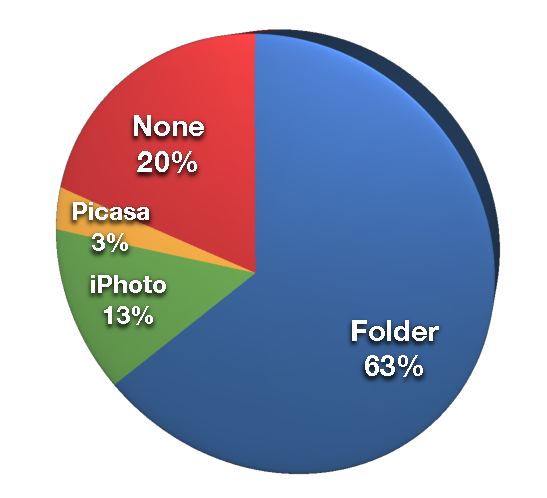
\includegraphics[width=\linewidth]{Figures/survey/organization}
	\end{center}
	\vspace{-20pt}
	\caption{Systematic organization in folders, in an application or no organization.}
	\vspace{-5pt}
	\label{fig:us:org}
\end{wrapfigure}

The question ``Do you have a systematic way to keep your photos organized?'' is meant to understand if people keep a system for their library, either on folders of inside an application.

Since most of the applications in the last question rely on folder organization, is no surprise that having a system in place for keeping things organized in folders is the clear winner of this question. Five people answered that they have this system inside an application and correlating this question with the previous one we found another expected aspect: only entry-level software is used to keep everything tidy, without touching folders, more exactly four people say they use iPhoto and one says Picasa is his/her choice.

20\% for the respondents claimed not having a way to organize their collections. The median of the number of photos of this group of people is 1050, the lowest, when compared to the other groups, the ones who use applications and the ones who rely on folders, both with 5000 of median.

% subsubsection systematic_organization (end)



\subsubsection{Photos in Close Sequence} % (fold)
\label{ssub:photos_in_close_sequence}

\begin{wrapfigure}{r}{0.3\textwidth}
	\vspace{-50pt}
	\begin{center}
		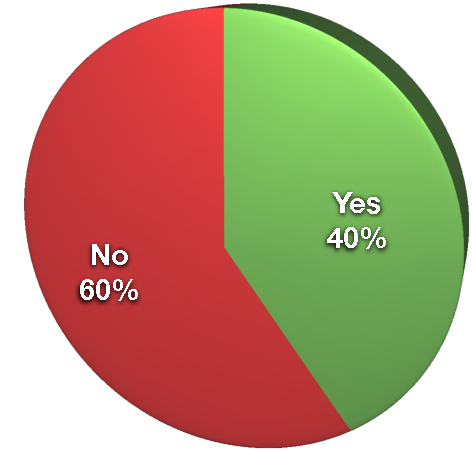
\includegraphics[width=\linewidth]{Figures/survey/close-seq}
	\end{center}
	\vspace{-20pt}
	\caption{Users that take photos in close sequence.}
	\vspace{-5pt}
	\label{fig:us:org}
\end{wrapfigure}


% subsubsection photos_in_close_sequence (end)


\red{Lorem ipsum dolor sit amet, consectetur adipisicing elit, sed do eiusmod tempor incididunt ut labore et dolore magna aliqua. Ut enim ad minim veniam, quis nostrud exercitation ullamco laboris nisi ut aliquip ex ea commodo consequat. Duis aute irure dolor in reprehenderit in voluptate velit esse cillum dolore eu fugiat nulla pariatur. Excepteur sint occaecat cupidatat non proident, sunt in culpa qui officia deserunt mollit anim id est laborum.
}
\vspace{\baselineskip}
\vspace{\baselineskip}
\vspace{\baselineskip}


\subsubsection{Preferred Features} % (fold)
\label{ssub:preferred_features}

\begin{wrapfigure}{r}{0.5\textwidth}
	\vspace{-50pt}
	\begin{center}
		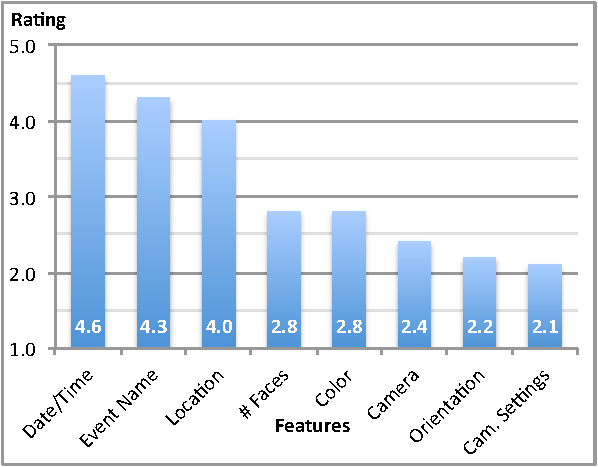
\includegraphics[width=\linewidth]{Figures/survey/features}
	\end{center}
	\vspace{-20pt}
	\caption{User rated features.}
	\vspace{-5pt}
	\label{fig:us:features}
\end{wrapfigure}

We had some ideas of what we would like to see extracted from the images and exposed to the user via our application and we asked for people's opinion on this survey and the results can be seen on \fig{us:features}.

While we weren't surprised by the favorites\linebreak Date/Time, Event and Location, we did expect\linebreak some higher ratings for number of faces and colors. Orientation and camera settings got the ratings we did expect.

% subsubsection preferred_features (end)



\subsubsection{Suggestions of Features} % (fold)
\label{ssub:suggestions_of_features}


De um conjunto de fotos semelhantes, ter um modelo com base em dados como:
- mais nitiida
- melhor color
- mais sorrisos
- mais olhos abertos
- etc.

.. possa classificar a melhor foto daquelas 4 ou 5 que tirámos ao nosso grupo de amigos por exemplo.
Format - RAW/JPEG; Original or edit; Number of Duplicates, Stored Location (disk C:/folder, etc)
Group by Tags, by faces, and intersect these groups...
Night or Day;
object/building/animal in the photo
person in the photo
Other EXIF Data
Single text field where i can browse for a particular/group of pictures with ease, by searching by the event name, or date.

I used to use people tagging, so I could easily find someone.
The faces of people.

% subsubsection suggestions_of_features (end)













% section characterization_of_photo_library (end)



\cleardoublepage

